\chapter{数据库设计}
\section{数据库环境说明}
本系统的数据系统采用MySQL数据库系统。

\section{数据库的命名规则}
只有标识符“ID”可以缩写,其他有意义的名词不允许缩写

表名统一用单数。命名最大字节数为100,关联表用该表"ID"作为外键

统一所有表无前缀

\section{逻辑设计}
数据库设计应满足BCNF范式

实体的逻辑关系图如下
\begin{figure}
    \centering
    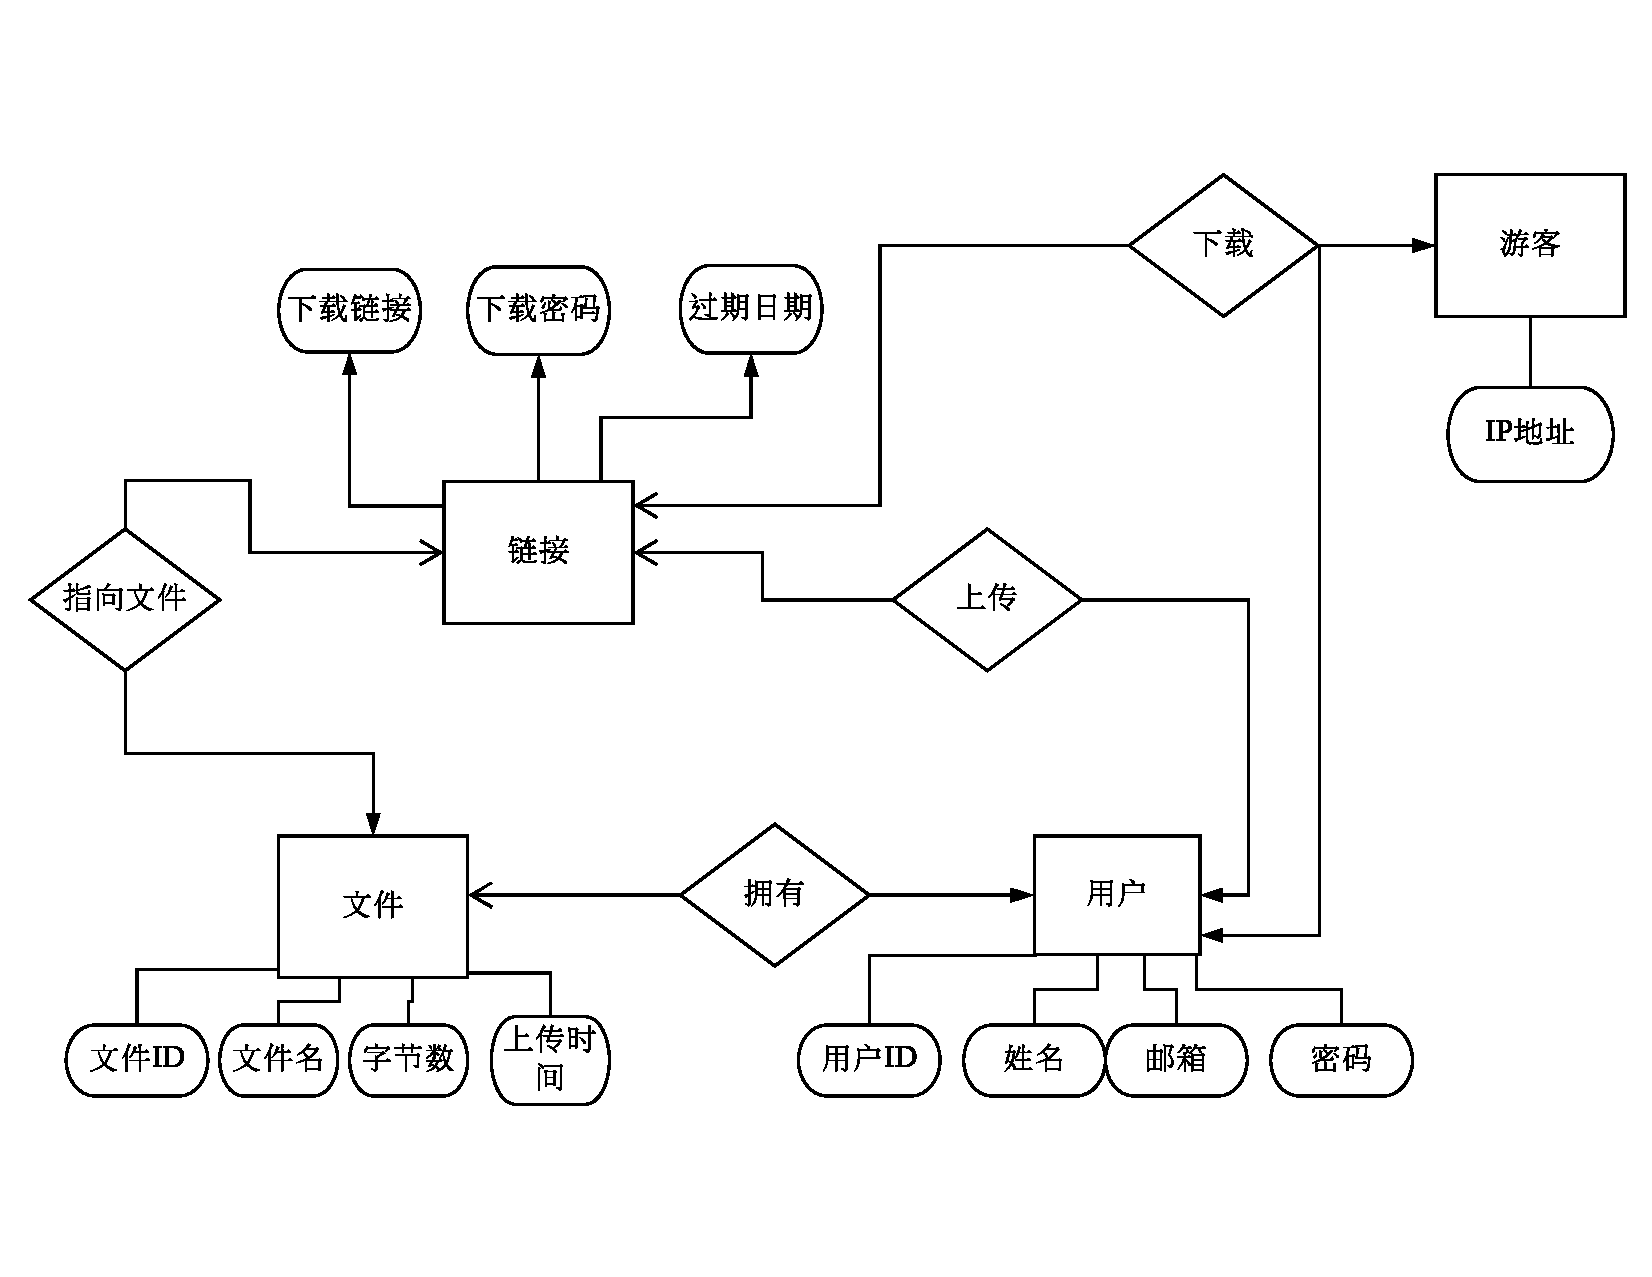
\includegraphics[width=16cm]{ER.pdf}
    \caption{ER关系图}\label{fig:noted-figure}
\end{figure}

\section{物理设计}
\subsection{数据库产品}
用哪家数据库,是否分布式等。
\subsection{实体属性、类型、精度}
\subsubsection{客户数据表设计}
\begin{table}[htbp]
\centering
\caption{用户数据表Users设计} \label{tab:client-database}
\begin{tabular}{|c|c|c|c|c|}
    \hline
    字段名 & 类型 & 大小 & 说明 & 备注 \\
    \hline
    ID & char & 64 & 用户的唯一标识符 & 主键\\
    \hline
    pw & char & 512 & 用户的登录密码 & · \\
    \hline
\end{tabular}
\note{用户数据表Users设计}
\end{table}

\subsubsection{订单数据表设计}
\begin{table}[htbp]
\centering
\caption{订单数据表Orders设计} \label{tab:order-database}
\begin{tabular}{|c|c|c|c|c|}
    \hline
    字段名 & 类型 & 大小 & 说明 & 备注 \\
    \hline
    ID & char & 64 & 订单的唯一标识符 & 主键\\
    \hline
    user & char & 64 & 对应用户 & 外键,来自xx表 \\
    \hline
\end{tabular}
\note{订单数据表Orders设计}
\end{table}
\section{安全性设计}
备份和容灾设计。

\section{数据库管理与维护说明}
对于数据库的维护,随时对数据库中的信息加以调试和保存备份。同样需要个工作人员进行系统的分析和用户的反馈,对系统进行升级以及功能的完善。同时保证系统安全有序的运行。